\section{Task 1 - Lexer}
\subsection{Explanation and Implementation}
The Lexer tokenizes the input stream by taking in character by character, grouping them into ordered tokens. A token is a tuple of (Lexeme, Attribute). A third attribute 'line number' is also added in the implementation for debugging purposes, both by the developer of the language as well as anyone using the language.

For the implementation, the entire file string is traversed and a vector of tokens is created. The reason for this is so that the file can be closed and the string discarded as soon as the lexer finishes. Any errors are reported by line number.

The following transition groups for the characters were chosen (This is also the Classifier Table):
\begin{enumerate}
	\item Singular punctuation (punctuation which exists on its own): + - ( ) \textbraceleft \textbraceright ; $\colon$ ,
	\item Exclamation point: !
	\item Fullstop: .
	\item Digit: 0-9
	\item Alpha: A-Z a-z \textunderscore
	\item Forward slash: /
	\item New-line: \textbackslash n
	\item Asterisk: *
	\item Equals: =
	\item Whitespace/tab or \textbackslash r: ' ' \textbackslash t \textbackslash r
	\item Greater/Smaller than: \textless  \textgreater
	\item Other: anything else
\end{enumerate}

The following diagram is the state transition diagram DFA. Note: 'not X' means any other character which is not X.
\begin{center}
\begin{figure}[H]
	\centering
	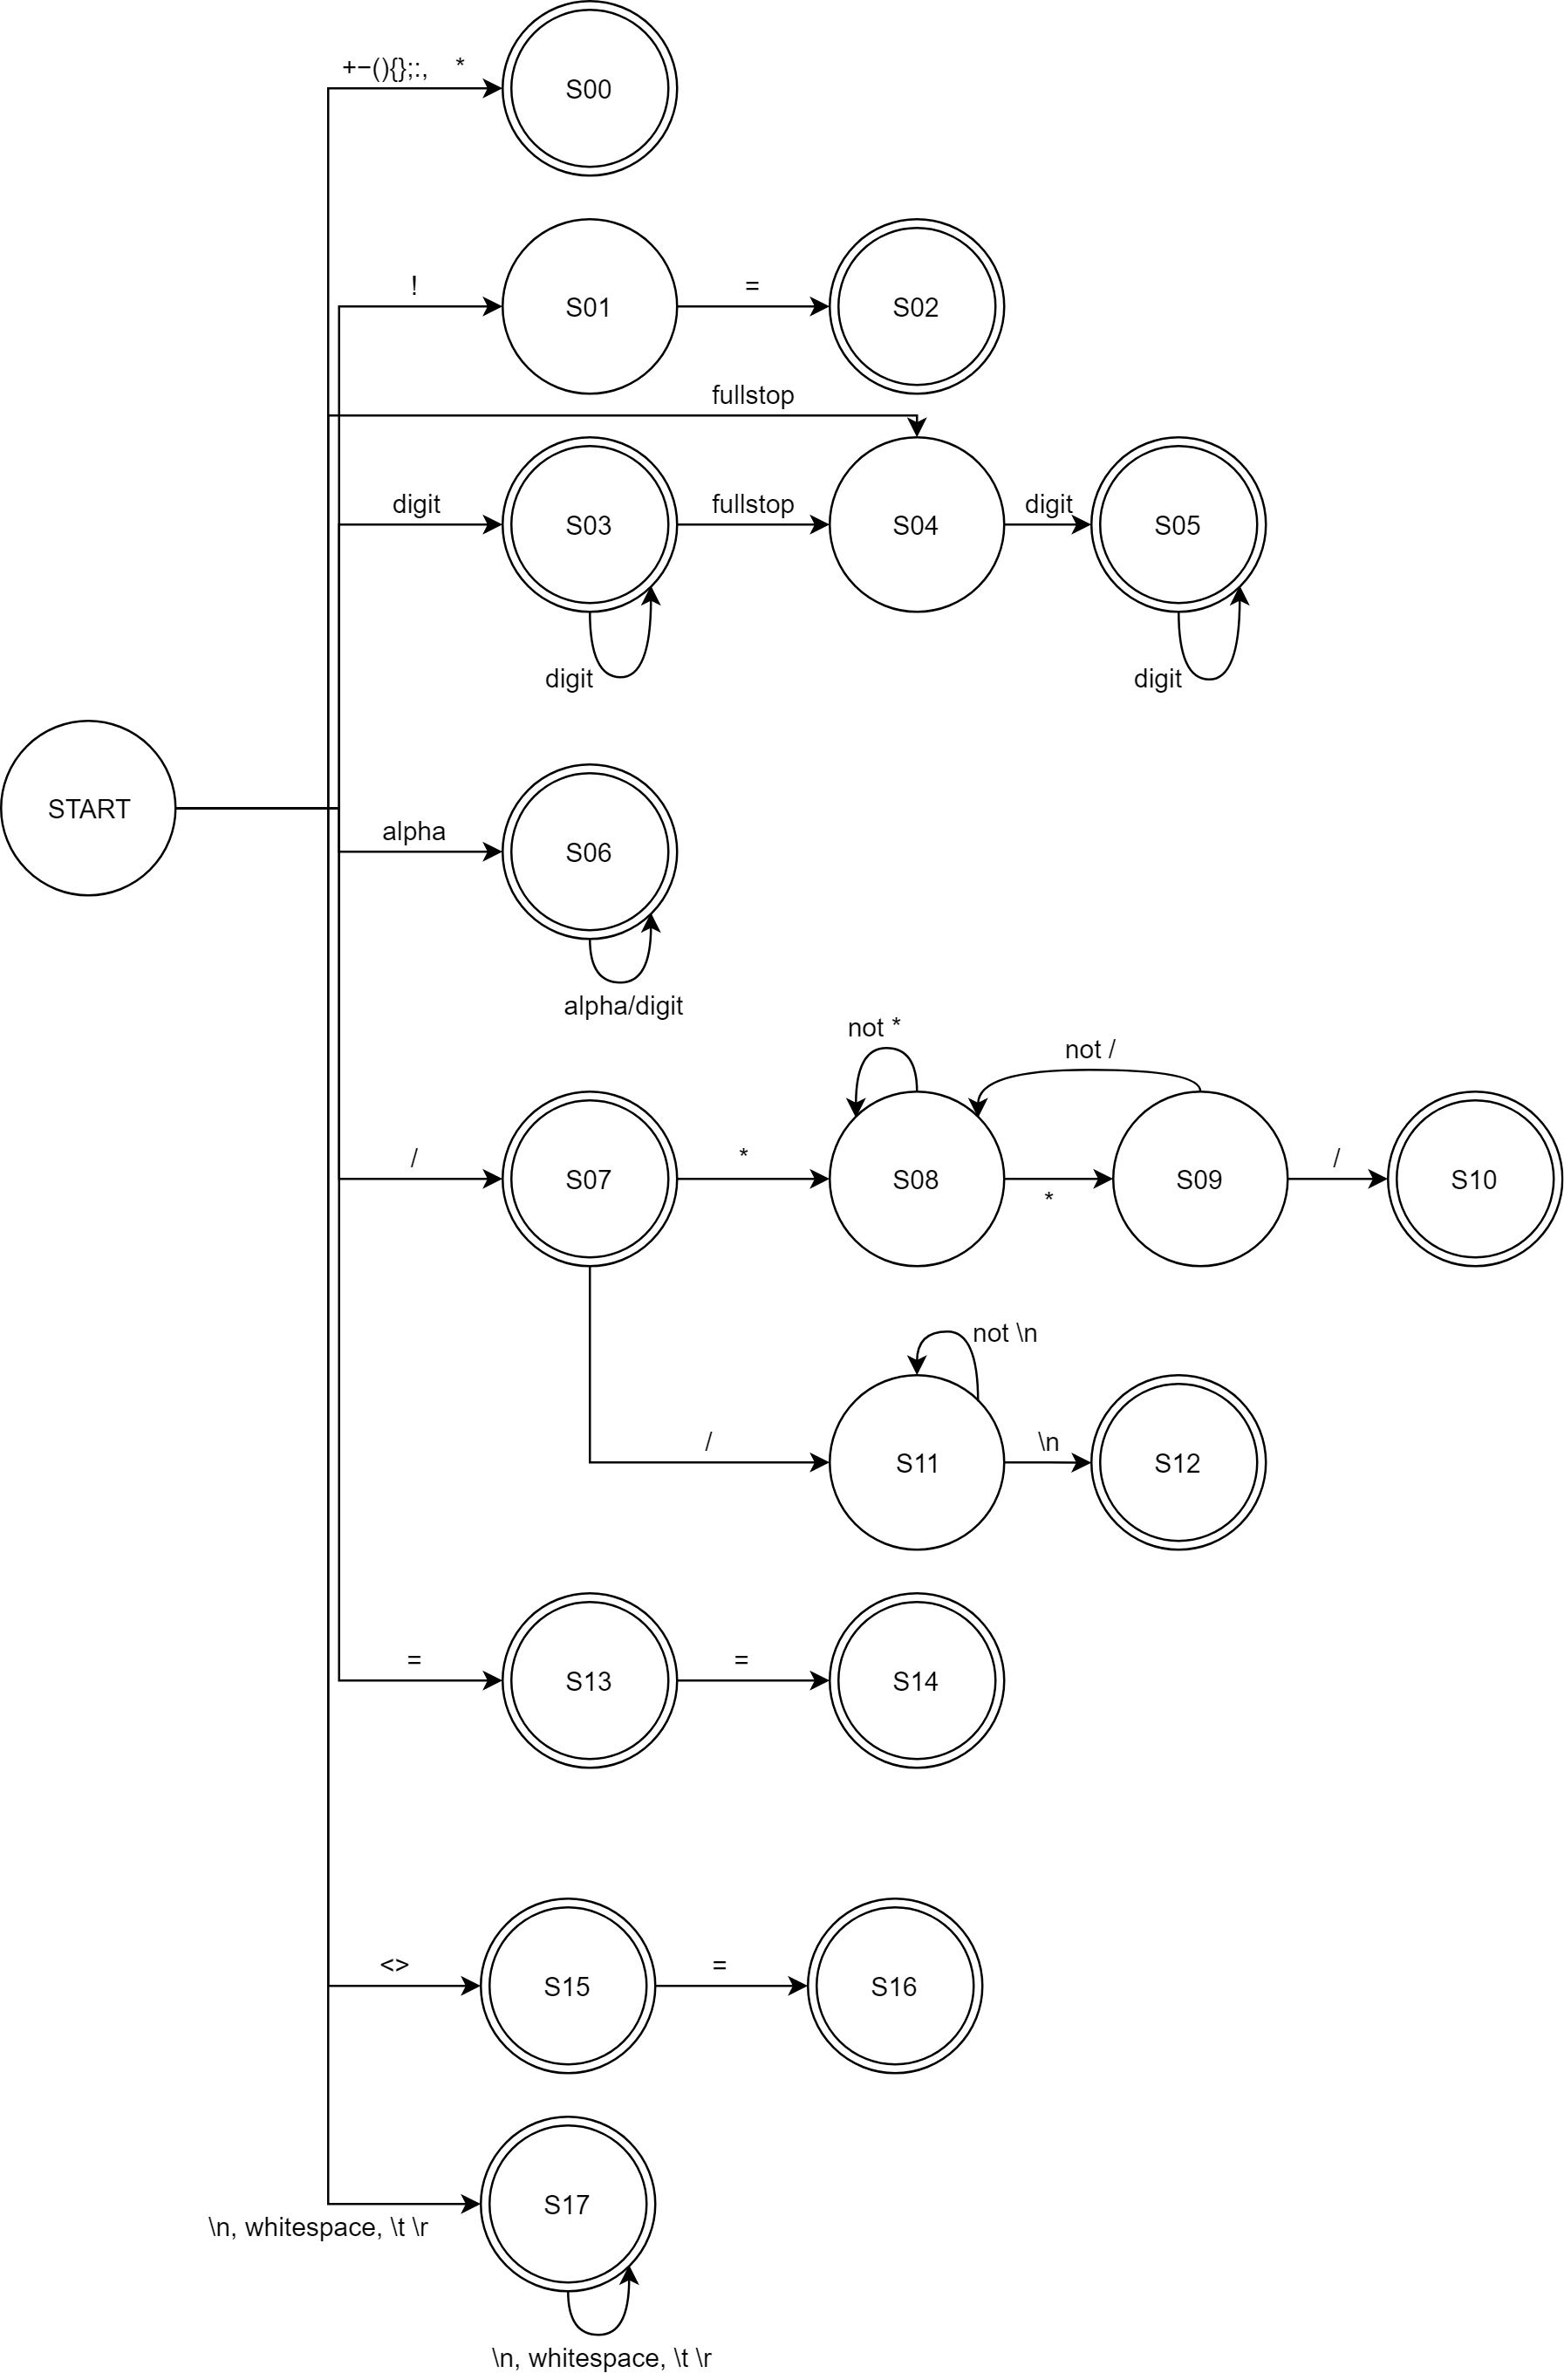
\includegraphics[scale=0.29]{Images/Q1_StateTransitionDiagram.png}
	\caption{DFA for Lexer}
\end{figure}
\end{center}

As a table, it looks like this in the code. The comments help to understand it better \cite{StateTransitionTable}:
\begin{figure}[H]
	\centering
	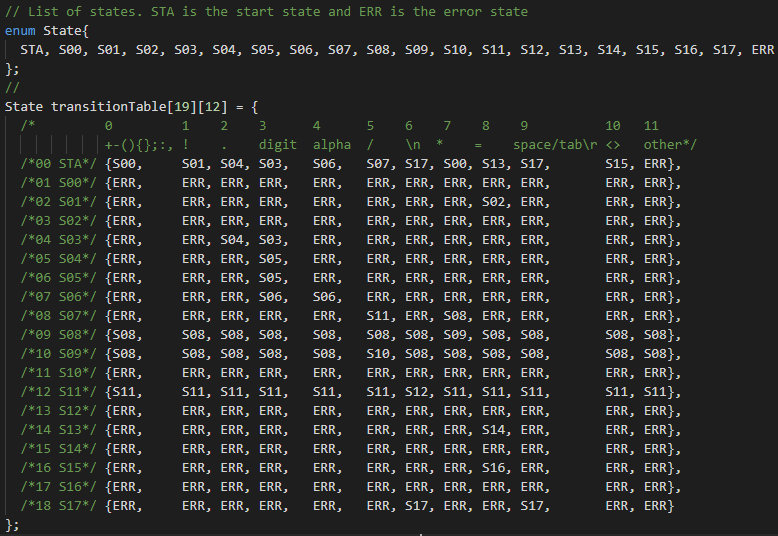
\includegraphics[width=\textwidth]{Images/Q1_StateTransitionTable.PNG}
	\caption{Table for Lexer}
\end{figure}

If the program goes to ERR (the error state), then the lexeme is over. If the current state is not a final state, then an error is reported and Lexical Analysis stops. If if the program goes to ERR and is in a final state, then the lexeme is kept and tokenized.

The token class is the following (Found in the Token.h file):
\begin{lstlisting}[language=C++]
class Token{
	public:
		static string TokenString[];
		// the Token parameters
		TokenType type;
		string lexeme = "";
		float number;
		int lineNumber;
		
		// constructor
		Token (TokenType _type, string _lexeme, float _number, int _lineNumber){
			type = _type;
			lexeme = _lexeme;
			number = _number;
			lineNumber = _lineNumber;
		}
		
		// helper method to neatly print the current token
		void printToken();
};
\end{lstlisting}

The final states result in some token. The following is a list of which states can result to which tokens (based on the lexeme).
\begin{enumerate}
	\item S0: PLUS, MINUS, OPEN\textunderscore BRACKET, CLOSED\textunderscore BRACKET, OPEN\textunderscore BRACE, CLOSED\textunderscore BRACE, COLON, SEMI\textunderscore COLON, COMMA, TIMES
	\item S2: NE
	\item S3: INT
	\item S5: FLOAT
	\item S6: ID (or one of mykeywords[] below)
	\item S7: DIVISION
	\item S11: discard '/*' and '*/' and return COMMENT
	\item S13: discard '//' and return COMMENT
	\item S14: EQ
	\item S15: EQQ
	\item S16: GT, ST
	\item S17: GE, SE
	\item S18: discard, since it is white spaces or new lines or tabs or carriage returns only
\end{enumerate}

\bigskip

The array of keywords in Token.cpp is as follows:
\begin{lstlisting} [language=C++]
// Used to check if a given string is a keyword (or identifier), and what type of keyword it is
struct keyword_token{
	string text;
	Token::TokenType tok_type;
};

keyword_token my_keywords[] = {
	{"and", AND},
	{"or", OR},
	{"not", NOT},
	{"if", IF},
	{"else", ELSE},
	{"for", FOR},
	{"while", WHILE},
	{"fn", FN},
	{"return", RETURN},
	{"bool", TYPE_BOOL},
	{"float", TYPE_FLOAT},
	{"int", TYPE_INT},
	{"var", VAR},
	{"true", BOOL},
	{"false", BOOL}
	{"print", PRINT}
};
\end{lstlisting}

The Lexer's \textit{Lex()} function does the following:
\begin{enumerate}
	\item Initialise state to the start state
	\item Initialise lexeme to the empty string
	\item Until EOF:
	\item \quad Read next character from the file
	\item \quad See to which column in the table this character points to, and use the current state as the row value to go to the new state
	\item \quad If at an error state
	\item \quad \quad Check if the the lexeme is valid with the previous state before the error state. If it is invalid, report the error, otherwise append the new token to the token vector, reset the lexeme and the state and go to step 3
	\item \quad else set the state as the one obtained from step 5 as the next state and append the character to the lexeme. Go back to step 3
\end{enumerate}

\subsection{Example Test}
Using the \textit{printToken()} in the \textit{Token} class \textit{printTokens()} method in the \textit{Lexer} class, when the following input is given to the program:
\begin{lstlisting}
someid true false 12.3 .4 56 89
< <= > >= == != and or not
= + - * /
if else for while fn return bool float int var
: ; ,
() {}
// hello world
/* hello 
world
2 */
\end{lstlisting}
The following output is printed from \textit{printTokens()}

\begin{figure}[H]
	\centering
	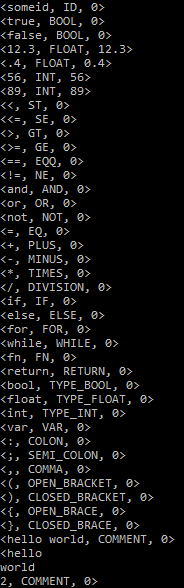
\includegraphics[scale=1]{Images/Q1_ExampleTest.png}
	\caption{Example output for the example input}
\end{figure}

